\documentclass{beamer}
\usetheme{metropolis}
\usepackage{graphicx}
\usepackage{subfig}
\usepackage{hyperref}
\usepackage{tcolorbox}
\title{Calculus-Based Physics-1: Mechanics (PHYS150-01): Week 5}
\date{October 2nd - October 6th, 2017}
\author{Jordan Hanson}
\institute{Whittier College Department of Physics and Astronomy}

\begin{document}
\maketitle

\section{Week 4 Review}

\begin{frame}{Week 4 Review}
\begin{enumerate}
\item Deep statements about physics: \textit{dynamics} and \textit{kinematics}
\begin{itemize}
\item \textbf{Lab activity}: Force, mass and stretching springs
\end{itemize}
\item Newton's \alert{First Law}
\begin{itemize}
\item \textbf{Lab activity}: force tables
\end{itemize}
\item Newton's \alert{Second Law}
\item Newton's \alert{Third Law}
\item Applications
\begin{itemize}
\item Free-body diagrams
\item Tension
\item Inclined surfaces
\item Restoring forces
\end{itemize}
\end{enumerate}
\end{frame}

\section{Week 4 Review Problems}

\begin{frame}{Week 4 Review Problems}
A powerful motorcycle can produce an acceleration of 3.50 m/s$^2$ while traveling at 90.0 km/h. At that speed the forces resisting motion, including friction and air resistance, total 400 N. (Air resistance is analogous to air friction. It always opposes the motion of an object.) What is the magnitude of the force the motorcycle exerts backward on the ground to produce its acceleration if the mass of the motorcycle with rider is 245 kg?
\begin{itemize}
\item A: 1260 N
\item B: 12,600 N
\item C: 960 N
\item D: 400 N
\end{itemize}
\end{frame}

\begin{frame}{Week 4 Review Problems}
Two teams of nine members each engage in a tug of war.  Each of the first team’s members has an average mass of 68 kg and exerts an average force of 1350 N horizontally. Each of the second team’s members has an average mass of 73 kg and exerts an average force of 1365 N horizontally.  What is magnitude of the acceleration of the two teams?  What is the tension in the section of rope between the teams?
\begin{itemize}
\item A: 0.106 m/s$^2$, 33435 N
\item B: 0.106 m/s$^2$, 12150 N
\item C: 0.955 m/s$^2$, 33435 N
\item D: 0.955 m/s$^2$, 12150 N
\end{itemize}
\end{frame}

\section{Week 5 Summary}

\begin{frame}{Week 5 Summary}
\begin{enumerate}
\item \alert{Motion in a circle}
\begin{itemize}
\item Constant velocity
\item Constant acceleration
\item \textit{Returning to this topic when we reach \alert{momenum}}
\end{itemize}
\item \alert{Friction}
\begin{itemize}
\item Normal force and friction
\item Static, kinetic
\end{itemize}
\item \alert{Drag}
\begin{itemize}
\item Terminal velocity
\end{itemize}
\item \alert{Restoring Forces}
\begin{itemize}
\item Hooke's Law
\item Young's modulus
\item Shear modulus
\item Bulk modulus
\end{itemize}
\end{enumerate}
\end{frame}

\section{Motion in a Circle}

\begin{frame}{Motion in a Circle}
\begin{figure}
\centering
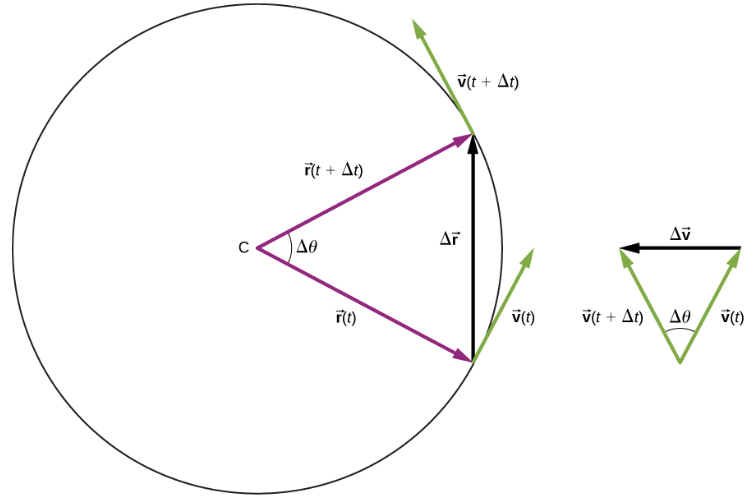
\includegraphics[width=0.9\textwidth]{figures/circle.png}
\caption{\label{fig:circle} A visual explanation of centripetal acceleration.}
\end{figure}
\end{frame}

\begin{frame}{Motion in a Circle}
\small
The triangle involving velocity is \textit{similar} to the triangle involving radii.  (Similar means ratios of side lengths are the same).  Thus:
\begin{align}
\frac{\Delta v}{v} &= \frac{\Delta r}{r} \\
\Delta v &= \frac{v}{r}\Delta r \\
\frac{\Delta v}{\Delta t} &= \frac{v}{r}\frac{\Delta r}{\Delta t} \\
\lim_{\Delta t \to 0} \frac{\Delta v}{\Delta t} &= \frac{v}{r} \lim_{\Delta t \to 0} \frac{\Delta r}{\Delta t}
\end{align}
\begin{equation}
\boxed{a_{\rm C} = \frac{v^2}{r}}
\end{equation}
This acceleration is a \textbf{vector}, oriented towards the \textit{center} of the circle.
\end{frame}

\begin{frame}{Motion in a Circle}
If there is a centripetal acceleration, then we may also define a centripetal \textit{force}, via Newton's Second Law:
\begin{equation}
\vec{F}_{\rm C} = m \frac{v^2}{r} \hat{r}
\end{equation}
Remember, this equation is meant to indicate a vector pointing towards the \textit{center of the circle}.
\end{frame}

\begin{frame}{Motion in a Circle}
One other kinematic variable: \textit{angular velocity} $\omega$, in radians per second.  If $v$ is the radial velocity, the velocity at the edge of the circle, then 
\begin{equation}
v = r\omega
\end{equation}
(From the definition of the radian).  Think of $\omega = \frac{d\theta}{dt}$.  Then the centripetal force is
\begin{equation}
F_{\rm C} = - m r \omega^2
\end{equation}
\end{frame}

\begin{frame}{Motion in a Circle}
A man swings from a 10 meter long rope, and the centripetal force balances the gravitational force.  What is the radial velocity of the man? ($g \approx 10$ m/s$^2$).
\begin{itemize}
\item A: 1 m/s
\item B: 5 m/s
\item C: 10 m/s
\item D: 20 m/s
\end{itemize}
\end{frame}

\begin{frame}{Motion in a Circle}
To prepare for the experience of launching away from Earth, astronauts train on centrifuges that simulate g-forces on their bodies.  Suppose a 50 kg astronaut is seated in a centrifuge that moves her in a circle with radius 10 meters.  At what radial velocity will the centripetal force reach 4 g's?  (Take the ratio of the centripetal force to the astronaut's weight).  Does the answer depend on the mass of the astronaut?
\begin{itemize}
\item A: 1 m/s, yes
\item B: 10 m/s, no
\item C: 20 m/s, yes
\item D: 20 m/s, no
\end{itemize}
\end{frame}

\begin{frame}{Motion in a Circle}
Notice that $\Delta \theta = \omega t$, just like one of our \textit{constant-velocity} type equations in linear kinematics.  We can therefore write the position vector of a system undergoing uniform circular motion as follows:
\begin{equation}
\vec{r}(t) = R\cos(\omega t) \hat{i} + R\sin(\omega t) \hat{j}
\end{equation}
(R is the radius of the circle).  We can refer to $\omega$ as the angular frequency of this function, and the system goes around the circle once per \textit{period}, or $T = 2\pi/\omega$.
\end{frame}

\begin{frame}{Motion in a Circle}
We can take derivatives to find that:
\begin{equation}
\vec{v}(t) = \frac{d\vec{r}(t)}{dt} = -R\omega\sin(\omega t) \hat{i} + R\omega\cos(\omega t) \hat{j}
\end{equation}
\begin{equation}
\vec{a}(t) = \frac{d\vec{v}(t)}{dt} = -R\omega^2\cos(\omega t) \hat{i} - R\omega^2\sin(\omega t) \hat{j}
\end{equation}
Notice that the acceleration is always negative, or a vector pointing towards the center of the circle.
\end{frame}

\begin{frame}{Motion in a Circle}
A proton has a speed $2 \times 10^6$ m/s and is moving in a circle in the x-y plane of radius 2 m.  What is the position of the proton at $t = 2 \times 10^{-6}$ seconds?  (At $t=0$, the proton is on the x-axis at $\vec{r}(t) = 2$ m $\hat{i}$).
\begin{itemize}
\item A: $\vec{r} = (2\cos(2)\hat{i} + 2\sin(2)\hat{j})$ m
\item B: $\vec{r} = (2\cos(4)\hat{i} + 2\sin(4)\hat{j})$ m
\item C: $\vec{r} = (\cos(2)\hat{i} + \sin(2)\hat{j})$ m
\item D: $\vec{r} = (\cos(2)\hat{i})$ m
\end{itemize}
\end{frame}

\section{Friction}

\begin{frame}{Friction}
Some definitions: \\
\begin{itemize}
\item \textit{\alert{Friction}} is a force that opposes relative motion between systems in contact.
\item \textit{\alert{Kinetic friction}} occurs between two systems that are in contact and moving relative to one another.
\item \textit{\alert{Static friction}} is occuring between two systems in contact but there is no motion.
\end{itemize}
\end{frame}

\begin{frame}{Friction}
\begin{figure}
\centering
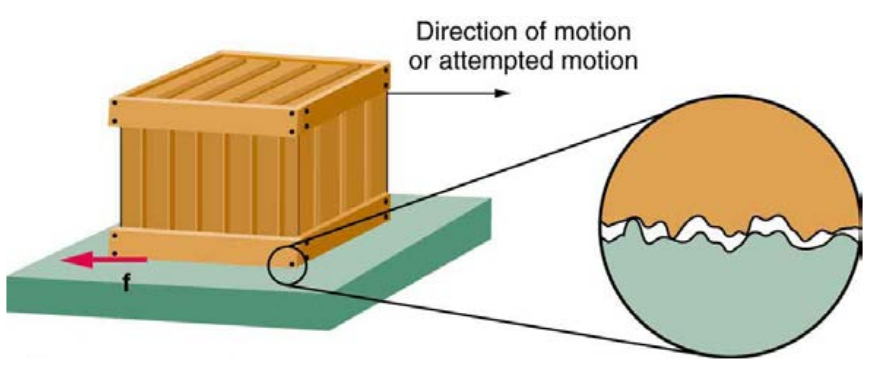
\includegraphics[width=0.8\textwidth]{figures/friction.png}
\caption{\label{fig:fric} Friction is ultimately a microscopic phenomenon.}
\end{figure}
\end{frame}

\begin{frame}{Friction}
Let $N$ be the normal force, and $f$ is the force of friction opposing motion. \\
\vspace{0.5cm}
Static friction: \\
\begin{equation}
f_{\rm s} \leq \mu_{\rm s} N
\end{equation}
Static friction maximum: \\
\begin{equation}
f_{\rm s,max} = \mu_{\rm s} N
\end{equation}
Kinetic friction: \\
\begin{equation}
\boxed{
f_{\rm k} = \mu_{\rm k} N ~~~ (\mu_{\rm k} < \mu_{\rm s})}
\end{equation}
\end{frame}

\begin{frame}{Friction}
\begin{figure}
\centering
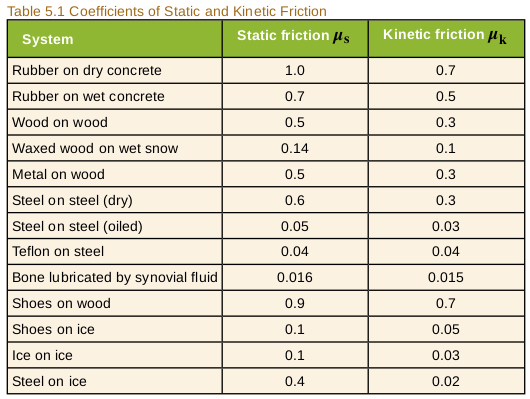
\includegraphics[width=0.8\textwidth]{figures/friction2.png}
\caption{\label{fig:fric2} A handy table of friction coefficients.  For example, compare ice and concrete.}
\end{figure}
\end{frame}

\begin{frame}{Friction}
Suppose an object is moving horizontally along a surface, experiencing gravity and a normal force but no other forces.  From Newton's second law, we have \\
\begin{align}
\vec{F}_{\rm net} &= m \vec{a} \\
\vec{f}_{\rm f} &= -m\vec{a} \\
-f_{\rm f}/m &= a \\
\mu_{\rm k} m g / m &= a \\
a &= \mu_{\rm k} g
\end{align}
We may think of the friction coefficient as the fraction of gravitational acceleration transduced into opposing motion.
\end{frame}

\begin{frame}{Friction}
What is the maximum frictional force in the knee joint of a person who supports 66.0 kg of her mass on that knee?  During strenuous exercise it is possible to exert forces to the joints that are easily ten times greater than the weight being supported. What is the maximum force of friction under such conditions?
\begin{itemize}
\item A: 1.06 N, 1.06 N
\item B: 0.157 N, 1.57 N
\item C: 103 N, 1033 N
\item D: 10.3 N, 103 N
\end{itemize}
\end{frame}

\begin{frame}{Friction}
Show that the acceleration of any object down a frictionless incline that makes an angle $\theta$ with the horizontal is $a = g\sin\theta$.  (Note that this is independent of mass).
\begin{figure}
\centering
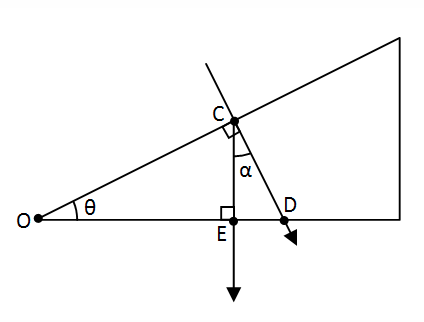
\includegraphics[width=0.4\textwidth]{figures/incline.png}
\caption{\label{fig:incline} Example of an incline with angle $\theta$ with respect to horizontal.}
\end{figure}
\end{frame}

\begin{frame}{Friction}
Next, show that the acceleration of any object down the same incline \alert{that has kinetic friction coefficient} $\mu_{\rm k} $ is given by $a = g(\sin\theta-\mu_{\rm k}\cos\theta)$.  Notice if we take the limit $\mu_{\rm k} \to 0$, we get the previous expression.
\begin{figure}
\centering
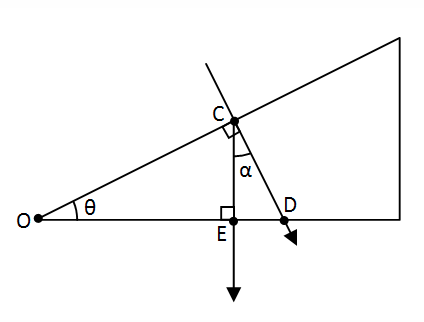
\includegraphics[width=0.4\textwidth]{figures/incline.png}
\caption{\label{fig:incline2} Now with friction!}
\end{figure}
\end{frame}

\begin{frame}{Friction}
A skiier is racing down a run with a 45 degree incline, and $\mu_{\rm k} = 0.1$.  Assuming the initial speed is 10 m/s, how long does it take to reach 40 m/s? (Let $g = 10$ m/s$^2$).
\begin{itemize}
\item A: $\approx 3\sqrt{2}$ seconds
\item B: $\approx 10\sqrt{2}/3$ seconds
\item C: $\approx 10$ seconds
\item D: $\approx 30$ seconds
\end{itemize}
\end{frame}

\section{Drag}

\begin{frame}{Drag forces}
\alert{The force of drag} resisting the motion of an object of cross-sectional area $A$ moving at velocity $v$ through a fluid with density $\rho$ is \\
\begin{equation}
\boxed{F_{\rm D} = \frac{1}{2}C\rho A v^2}
\label{eq:drag}
\end{equation}
In Eq. \ref{eq:drag}, C is a measured coefficient.
\end{frame}

\begin{frame}{Drag}
A professor is riding his bicycle to work, at a constant velocity of 10 m/s.  His cross-sectional area is 1.0 m$^2$, the density of air is $\rho = 1.2$ kg/m$^3$, and $C \approx 0.5$.  What is the force of drag?  If he ducks down, making his area 0.25 m$^2$, what is the new force of drag?
\begin{itemize}
\item A: 30 N, 7.5 N
\item B: 15 N, 15 N
\item C: 30 N, 30 N
\item D: 3 N, 3/4 N
\end{itemize}
\end{frame}

\begin{frame}{Drag: Terminal Velocity}
\small
Suppose an object is falling through the atmosphere of Earth.  At a certain speed, the object stops accelerating.  Why?  The force of \textit{drag balances the force of gravity}.  Draw a free-body diagram describing the situation.  If $m$ is the mass of the falling object, $g$ is the acceleration of gravity, $C$ is the drag coefficient from Eq. \ref{eq:drag}, $\rho$ is the density of air, and $A$ is the area of the object, show that the maximum speed reached is $v_{\rm T} = \left(\frac{2mg}{C\rho A}\right)^{1/2}$.  What is the terminal velocity of a skydiver with: $m = 64$ kg, $A = 0.5$ m$^2$, $g = 10$ m/s$^2$, $C \approx 1$, $\rho \approx 1$ kg/m$^3$?
\begin{itemize}
\item A: 1800 km/hr
\item B: 180 km/hr
\item C: 18 km/hr
\item D: 80 m/s
\end{itemize}
\end{frame}

\begin{frame}{Drag: Stoke's Law}
\small
\alert{\textbf{Stoke's Law}} describes drag on small systems moving slowly through viscous media: $F_{\rm D} = 6\pi r\eta v$, where $r$ is the radius of the object, $v$ is the velocity, and $\eta$ is the \textit{viscosity} (kg/(s$\cdot$m)).  In the same fashion as the prior exercise, show that the terminal velocity is $v_{\rm T} = mg/6\pi\eta v$.  Calculate this velocity assuming: $m\approx 10^{-9}$ kg, $r\approx 2 \cdot 10^{-3}$ m, $g\approx 10$ m/s$^2$, and $\eta \approx 2 \cdot 10^{-5}$ kg/(s m) for air.
\begin{itemize}
\item A: 100 cm/s
\item B: 10 cm/s
\item C: 1 cm/s
\item D: 1 mm/s
\end{itemize}
\end{frame}

\section{Restoring Forces}

\begin{frame}{Restoring Forces}
Let $F_{\rm app}$ be an applied force on a system, causing the length of the system to change by $\vec{x}$.  By Newton's Third Law, the system will exert a force $F$ in reaction. \\
\vspace{1cm}
\begin{tcolorbox}[colback=white,colframe=red!40!blue,title=Hooke's Law]
\alert{$\vec{F} = -k\vec{x}$}
\end{tcolorbox}
\vspace{0.5cm}
Hooke's Law is an example of a \textit{restoring force}.  Examples of systems that obey Hooke's Law are springs, pendula, and other oscillators.
\end{frame}

\begin{frame}{Restoring Forces: Oscillations...}
If a system follows Hooke's Law and Newton's Second Law in one-dimension, then \\
\begin{align}
m \frac{d^2x}{dt^2} &= -k x(t) \label{eq:osc1} \\
\frac{d^2x}{dt^2} &= -\frac{k}{m} x(t) \label{eq:osc2}
\end{align} \\
What set of functions obeys this differential equation?  Sines and cosines...
\end{frame}

\begin{frame}{Restoring Forces: Young's Modulus}
Suppose a force $F$ is \textit{applied} to a system of length $L$ and cross-sectional area $A$, which compresses an amount $x$.  Let \textit{Young's Modulus} be defined by $Y = k \frac{L}{A}$.  Rearranging Hooke's Law  gives \\
\begin{equation}
\frac{x}{L} = \frac{1}{Y}\frac{F}{A}
\end{equation}
\vspace{0.5cm}
Force applied per unit area is also known as \textit{pressure}, $p$.
\begin{equation}
\boxed{\frac{x}{L} = \frac{p}{Y}}
\label{eq:young}
\end{equation} \\
The SI unit for pressure is the \textit{Pascal}, or 1 Newton per square meter.  Young's Modulus also applies to tension, or the opposite of linear compression.
\end{frame}

\begin{frame}{Restoring Forces: Young's Modulus}
\begin{figure}
\centering
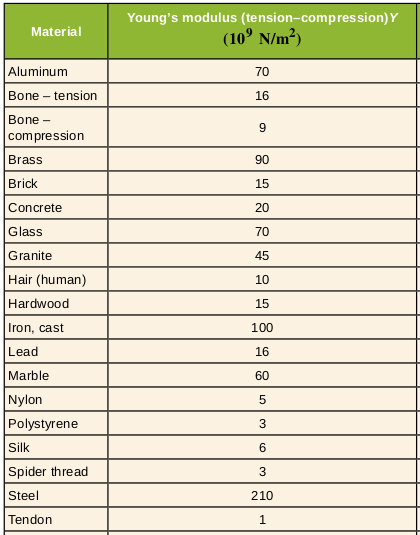
\includegraphics[width=0.45\textwidth]{figures/young.png}
\caption{\label{fig:young} Table of Young's Modulii for different materials.}
\end{figure}
\end{frame}

\begin{frame}{Restoring Forces: Young's Modulus}
Young's Modulus for spider silk is $3 \times 10^9$ N/m$^2$.  If a spider weighs 1 mg, and dangles from a strand of its silk with radius 0.5 mm, by what fraction does the strand stretch?  (Hint: this fraction is $x/L$ in Eq. \ref{eq:young}).
\begin{itemize}
\item A: $4 \times 10^{-2}$
\item B: $4 \times 10^{-3}$
\item C: $4 \times 10^{-5}$
\item D: $4 \times 10^{-9}$
\end{itemize}
Why is it important for the silk of the spider to be this strong, from the perspective of evolution?
\end{frame}

\begin{frame}{Restoring Forces: Young's Modulus}
Suppose we had a rope made of spider silk (same number for Young's Modulus), with a radius of 0.5 cm.  By what fraction would this rope stretch if it were to support the weight of a 80 kg human?
\begin{itemize}
\item A: $10^{-3}$
\item B: $10^{-9}$
\item C: $10^{-7}$
\item D: $10^{-4}$
\end{itemize}
Yep, spider silk can hold a person without breaking.  Just need the right thickness.
\end{frame}

\begin{frame}{Restoring Forces: Stress and Strain}
Pressure, when applied to material solids, is also called \textit{stress}.  The fractional change in length of a material solid, $x/L$ (or $\Delta L/L_{\rm 0}$ in the text), is called the \textit{strain}.  Using Eq. \ref{eq:young}, we have
\begin{equation}
stress = Y \times strain
\end{equation}
$Y$ is just the coefficient relating the linear shape change to the applied pressure.  Other coefficients describe other shape changes...
\end{frame}

\begin{frame}{Restoring Forces: Shear Modulus}
Suppose the applied force is \textit{perpendicular} to $L$ and \textit{parallel} to $A$, also known as \textit{shearing}.  The \textit{Shear Modulus} $S$ relates shear to stress: \\
\begin{equation}
stress = S \times shear
\end{equation}
Shear and strain are similar, but in different directions.  One critical example is human bone.
\end{frame}

\begin{frame}{Restoring Forces: Shear Modulus}
Suppose the ratio of Young's Modulus for bone to the Shear Modulus for bone is 20:1: $Y/S = 20$.  Leg bone can withstand stresses that lead to strains of $10^{-3}$ before breaking.  Suppose that corresponds to a pressure of $10^6$ N/m$^2$.  What pressure applied to a bone sideways (shear) would lead to a fracture?
\begin{itemize}
\item A: $\frac{1}{2} \times 10^{5}$ N/m$^2$
\item B: $\frac{1}{2} \times 10^{4}$ N/m$^2$
\item C: $\frac{1}{2} \times 10^{3}$ N/m$^2$
\item D: $\frac{1}{2} \times 10^{2}$ N/m$^2$
\end{itemize}
\end{frame}

\begin{frame}{Restoring Forces: Shear Modulus}
If that pressure was applied to a $2$ cm$^2$ area of leg ($2 \times 10^{-2}$ cm$^2$), what is the corresponding force?
\begin{itemize}
\item A: $10^{3}$ N
\item B: $10^{5}$ N
\item C: $10^{2}$ N
\item D: $10^{3}$ N
\end{itemize}
How does this compare to your body weight? Is it much greater, about the same, or less?  What if someone stood on your leg with one foot.  Would that break your leg?
\end{frame}

\begin{frame}{Restoring Forces: Bulk Modulus}
Suppose the applied force per unit area is just some constant pressure, $p$, coming from all directions uniformly.  The \textit{Bulk Modulus} $B$ relates fractional volumetric change to this pressure: \\
\begin{equation}
p = B\frac{\Delta V}{V}
\end{equation}
\end{frame}

\begin{frame}{Restoring Forces: Shear Modulus}
The bulk modulus of brass is about $75 \times 10^{9}$ N/m$^2$.  Suppose we want to compress a brass sphere of volume 4.3 cm$^3$ into a ring of volume 2.15 cm$^3$.  What pressure is required?
\begin{itemize}
\item A: $2.15 \times 10^{9}$ N/m$^2$ 
\item B: $37.5 \times 10^{6}$ N/m$^2$ 
\item C: $37.5 \times 10^{9}$ N/m$^2$ 
\item D: $75 \times 10^{9}$ N/m$^2$ 
\end{itemize}
How does this compare to atmospheric pressure, if 1 atmosphere is 100 kPa = $10^5$ N/m$^2$?
\end{frame}

\section{Warm-up problems (Review for Midterm)}

\begin{frame}{Warm-up problems (Review for Midterm)}
\small
\begin{align}
\vec{a} &= 3\hat{i} + 4\hat{j} \\
\vec{b} &= 6\hat{i} + 8\hat{j}
\end{align}
\alert{Stand up!} On the boards in your groups, work out the following:
\begin{itemize}
\item What is the magnitude of $\vec{a}$?
\item What is the magnitude of $\vec{b}$?
\item What is $\vec{a} \cdot \vec{b}$?
\item What is the angle between these vectors?  (Use the formula involving the dot product).
\item What is the angle between these vectors? (Determine by drawing a graph).
\item What is $\vec{c} = \vec{b}-\vec{a}$?  Draw $\vec{c}$.
\end{itemize}
\end{frame}

\section{Measuring Coefficients of Friction}

\begin{frame}{Measuring Coefficients of Friction}
\begin{itemize}
\small
\item The goal of this lab activity is to measure the coefficient of \textit{static friction}, $\mu_{\rm s}$.  In your lab notebook, describe in words the difference between kinetic and static friction.
\item The setup looks like this:
\begin{figure}
\centering
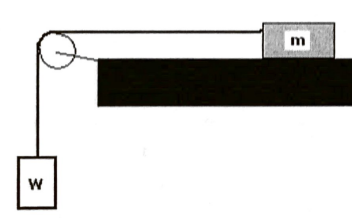
\includegraphics[width=0.3\textwidth]{figures/slide.png}
\end{figure}
\item We can apply a known force to the block of mass $m$ ($125\pm5$ grams) by adding weights to the end of the string hanging over the frictionless pulley.  (\textbf{Measure the mass of the wood block using the spring-scales}).  Record the mass in your lab notebook.
\item In your lab notebook, draw a free body diagram, where the \textit{system} is the wood block.
\end{itemize}
\end{frame}

\begin{frame}{Measuring Coefficients of Friction}
\begin{itemize}
\small
\item Progressively add small amounts of weight to the end of the pulley, and record the minimum amount of mass required to get the pulley moving.
\item Now increase the mass of the wooden block by adding 200 grams on top of it.  Repeat the procedure, recording the minimum mass on the pulley required to cause sliding.
\item Now increase the mass of the wooden block by adding another 200 grams.  Repeat the procedure.
\item Graph the pulley \textbf{force} versus the \textbf{force}, and calculate the slope.  The slope should be equal to $\mu_{\rm s}$.  Explain this using the free-body diagram.
\end{itemize}
\end{frame}

\section{Conclusion}

\begin{frame}{Week 5 Summary}
\begin{enumerate}
\item \alert{Friction}
\begin{itemize}
\item Normal force and friction
\item Static, kinetic
\end{itemize}
\item \alert{Drag}
\begin{itemize}
\item Terminal velocity
\end{itemize}
\item \alert{Restoring Forces}
\begin{itemize}
\item Hooke's Law
\item Young's modulus
\item Shear modulus
\item Bulk modulus
\end{itemize}
\end{enumerate}
\end{frame}

\section{Answers}

\begin{frame}{Answers}
\begin{columns}[T]
\begin{column}{0.5\textwidth}
\begin{itemize}
\item 1260 N
\item 0.106 m/s$^2$, 12150 N
\item 10 m/s
\item 20 m/s, no
\item $\vec{r} = (2\cos(2)\hat{i} + 2\sin(2)\hat{j})$ m
\item 10.3 N, 113 N
\item $10\sqrt{2}/3$ seconds
\item 30 N, 7.5 N
\item 180 km/hr
\item 1 cm/s
\end{itemize}
\end{column}
\begin{column}{0.5\textwidth}
\begin{itemize}
\item $4 \times 10^{-9}$
\item $10^{-3}$
\item $\frac{1}{2} \times 10^{5}$ N/m$^2$
\item $10^{3}$ N
\item $37.5 \times 10^{9}$ N/m$^2$ 
\end{itemize}
\end{column}
\end{columns}
\end{frame}

\end{document}
